\chapter{Concept - Keeping Information Secret}
\label{chapter:keepingInformationSecret}

Ciphers have been used for thousands of years \cite{HistoryOfCryptography}. They are used to keep information secret from people, that are not supposed to have knowledge of it. Non-encrypted information is called clear text. Once a clear text is encrypted, it is called a cipher text and only people who know the decryption procedure for the cipher text can read the originally encrypted information.
The exercises in this section introduce pupils to the concepts of cryptography. Simple nouns are used as clear text.

\section{Cipher Texts from Reversed Letters}
\label{section:patterns}

\subsection{Exercises}
The cipher used in these exercises is a simple mixture of letters. Both encryption and decryption are trained. In the decryption exercise, the pattern used for encryption is shown. The pupils need to understand the pattern and move the letters in the cipher text accordingly to obtain the clear text. The encryption exercise is set up the other way around. The pupils see the clear text and need to move letters according to the pattern to generate the cipher text. Both encryption and decryption exercises have two difficulty levels. They differ by the amount of tuples:

\begin{itemize}
    \item \textbf{easy} - one tuple, i.e two swapped letters 
    \item \textbf{medium} - two tuples, i.e in total four swapped letters if the the word has at least four letters, otherwise only two swapped letters 
\end{itemize}

\begin{example}
    The cipher text is \code{TNOAM} and the pattern is shown in figure \ref{fig:pattern} (easy level). By moving the letter in the cipher text according to the pattern, the clear text can be retrieved: \code{MONAT}.
\end{example}

\begin{figure} 
    \centering
    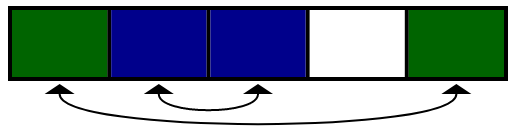
\includegraphics[width=0.4 \columnwidth]{figures/pattern.png}
    \caption{Pattern} 
    \label{fig:pattern} 
\end{figure}

\subsection{Implementation}

Both exercises have a similar implementation. Both need a drawn pattern that indicates the cipher. Fundamentally, the only difference is that, for the decryption exercise, the given text consists of reversed letters and the solution is compared to the original word, while the encryption exercise gives first the original word as a text and the solution is compared to match the pattern (figures \ref{fig:patternDecryption} and \ref{fig:patternEncryption}). 
The pattern is created by generating an array of tuples. Each tuple indicates two swapped letters. These two letters are selected randomly and have to be distinct. The exact algorithm used is given in listing \ref{lst:createPattern}.

%TC:ignore
\begin{lstlisting}[language=TypeScript,caption={Algorithm to generate an array of distinct tuples of given size},label={lst:createPattern}]
createPattern(text: string[], swapAmount: number): Array<[number, number]> {
  const pattern = new Array<[number, number]>();
  const letters = [...Array(text.length).keys()];
  for (let j = 1; j <= swapAmount && 2 * j <= text.length; j++) {
    const leftIndex = Math.floor(Math.random() * letters.length);
    const left = letters[leftIndex];
    letters.splice(leftIndex, 1);
    const rightIndex = Math.floor(Math.random() * letters.length);
    const right = letters[rightIndex];
    letters.splice(rightIndex, 1);
    pattern.push([Math.min(left, right), Math.max(left, right)]);
  }
  return pattern;
}
\end{lstlisting}
%TC:endignore

The array of tuples needs to be graphically represented. For this purpose, the HTML \code{canvas} element is used. A \code{canvas} element is a two-dimensional area, where one can draw diagrams, edit images and create animations with the help of a scripting language like JavaScript or TypeScript. A \code{canvas} element has a height and width and is basically a coordinate system with the origin in the top left corner at (0, 0). Usually 1 unit corresponds to 1 pixel and all elements are drawn relative to the origin. Some examples of basic operations on a \code{canvas} element are drawing straight lines, curves and moving the pen without drawing. Additionally, one can choose to either fill the drawn structure with a color or only highlight its border \cite{MDNWebDocs}. These operations already meet the requirements to draw a pattern. The implementation is given in  listing \ref{lst:createPattern} and can be broken down to four steps: 

\begin{itemize}
  \item \textbf{drawing the grid} - each cell represents a letter of the word
  \item \textbf{colorizing the pairs} - the pairs representing the two letters that need to be swapped are colorized in the same color
  \item \textbf{drawing the arrow heads} - below each cell, that is part of a pair, an arrow head is drawn
  \item \textbf{drawing the arrow lines} - connecting the pairs with lines without the lines overlapping or unnecessarily crossing each other
\end{itemize}

Everything drawn outside of the \code{canvas} element border is invisible, hence special attention needs to be payed to the first few lines in listing \ref{lst:createPattern} (L 2-5). Each drawn line has a width. When a line starting at the origin is drawn horizontally, half of the lines are outside of the \code{canvas} element border and hence not visible. Therefore, the rectangle is drawn with a distance of half a line width to the actual border of the \code{canvas} element, so the whole line width is drawn instead of only half of it. 

Creating the grid requires creating a rectangle, giving the shape first and then the lines creating the cells. To draw the lines, the pen needs to be moved to the start of the line, set down, moved to the end of the line and finally be drawn (listing \ref{lst:drawGrid}). 

Drawing an arrow head includes more operations. The pen is first moved to the pointy end of the arrow, set down, moved to the two other corners and back to the pointy end. This time, instead of only highlighting just the border, the whole structure is filled black (listing \ref{lst:drawArrowHead}).

%TC:ignore
\begin{lstlisting}[language=TypeScript,caption={Implementation to draw the pattern on a canvas element},label={lst:drawPattern}]
drawPattern(cells: number, pairs: [number, number][]) {
  const rectX = this.lineWidth / 2;
  const rectY = this.lineWidth / 2;
  const rectWidth = this.width - this.lineWidth;
  const cellHeight = this.height / 2 - this.lineWidth;
  const cellWidth = rectWidth / cells;

  this.drawGrid(rectX, rectY, rectWidth, cellHeight, cells, cellWidth);

  // sort to have it easier to draw the lines connecting the boxes on the correct height
  pairs.sort(([a, b], [c, d]) => Math.abs(a - b) - Math.abs(c - d));
  const arrowLevelY = this.calculateArrowLevelY(pairs);
  for (let i = 0; i < pairs.length; i++) {
    for (let j = 0; j < 2; j++) {
      const pairIndex = pairs[i][j];

      this.ctx.fillStyle = this.colors[i % this.colors.length];
      this.fillBox(rectX, rectY, cellHeight, cellWidth, pairIndex);

      const centerX = rectX + cellWidth * pairIndex + cellWidth / 2;
      this.ctx.fillStyle = "black";
      this.drawArrowHead(
        centerX,
        rectY + cellHeight + 5,
        Math.min(30, cellWidth),
        10
      );
    }

    this.drawArrowLine(
      cellHeight,
      cellWidth,
      rectY,
      rectX,
      arrowLevelY.get(JSON.stringify(pairs[i])),
      cells,
      pairs[i]
    );
  }
}
\end{lstlisting}
%TC:endignore

%TC:ignore
\begin{lstlisting}[language=TypeScript,caption={},label={lst:drawGrid}]
drawGrid(
  rectX: number,
  rectY: number,
  rectWidth: number,
  cellHeight: number,
  cells: number,
  cellWidth: number
) {
  // draw box
  this.ctx.strokeRect(rectX, rectY, rectWidth, cellHeight);
  // draw walls
  for (let i = 1; i < cells; i++) {
    this.ctx.beginPath();
    this.ctx.moveTo(rectX + cellWidth * i, rectY);
    this.ctx.lineTo(rectX + cellWidth * i, rectY + cellHeight);
    this.ctx.stroke();
  }
}
\end{lstlisting}
%TC:endignore

%TC:ignore
\begin{lstlisting}[language=TypeScript,caption={},label={lst:drawArrowHead}]
drawArrowHead(
  headX: number,
  headY: number,
  headWidth: number,
  headHeight: number
) {
  this.ctx.beginPath();
  this.ctx.moveTo(headX, headY);
  this.ctx.lineTo(headX - headWidth / 2, headY + headHeight);
  this.ctx.lineTo(headX + headWidth / 2, headY + headHeight);
  this.ctx.lineTo(headX, headY);
  this.ctx.fill();
}
\end{lstlisting}
%TC:endignore

\begin{example}
  The pattern in figure \ref{fig:pattern} is generated by calling \code{drawPattern} with \code{5} as \code{cells} and \code{[[0, 4], [1, 2]]} as \code{pairs}.
  %TC:ignore
  \begin{lstlisting}[language=TypeScript]
    drawPattern(5, [[0, 4], [1, 2]])
  \end{lstlisting}
  %TC:endignore
\end{example}

\begin{figure} 
    \centering
    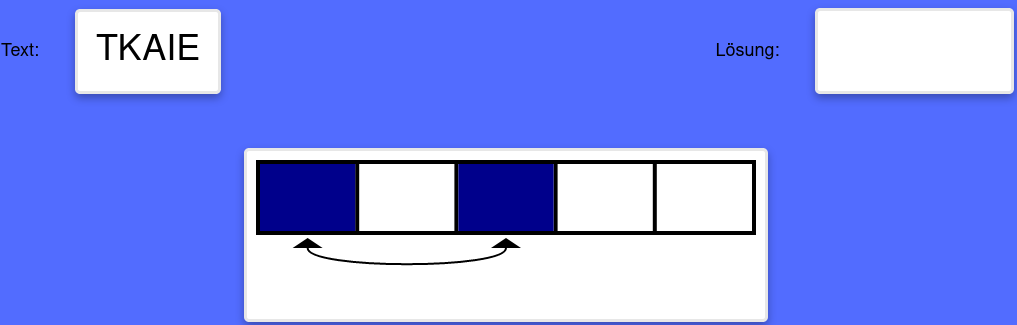
\includegraphics[width=1.0 \columnwidth]{figures/pattern_decrypt.png}
    \caption{Pattern decryption exercise} 
    \label{fig:patternDecryption} 
\end{figure}

\begin{figure} 
    \centering
    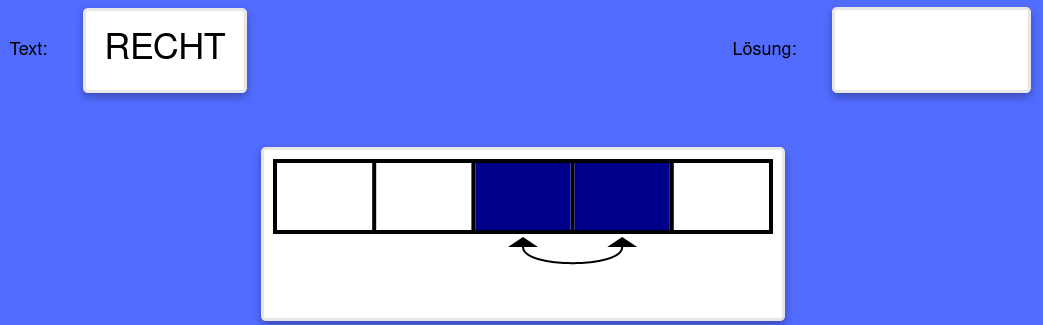
\includegraphics[width=1.0 \columnwidth]{figures/pattern_encrypt.png}
    \caption{Pattern encryption exercise} 
    \label{fig:patternEncryption} 
\end{figure}

\section{Cipher Texts from New Characters}
\label{section:symbols}

\subsection{Exercises}
Sometimes, only moving symbols is not enough to keep information secret. A better way is to substitute symbols with new symbols. These symbols may be letters, numbers or completely new symbols, that are solely invented for the purpose of encrypting information.
In the following exercises the last approach is followed. Again both directions, encryption and decryption, are trained. But this time, instead of having a pattern, there is a symbol table showing how the numbers or letters are encrypted. The decryption exercise has two difficulty levels:

\begin{itemize}
    \item \textbf{easy} - use symbol table with numbers
    \item \textbf{medium} - use symbol table with letters
\end{itemize}

\begin{example}
    The cipher text is shown in figure \ref{fig:cipher_number} and the symbol table in figure \ref{fig:symboltable_numbers}. By using the symbol table one can decrypt the cipher text to \code{52}.
\end{example}

\begin{figure}[h]
    \centering
    
\includegraphics[width=0.15\columnwidth]{figures/cipher_number.png}
    \caption{Cipher text of encrypted numbers}
    \label{fig:cipher_number} 
\end{figure}
\begin{figure}[h]
    \centering
    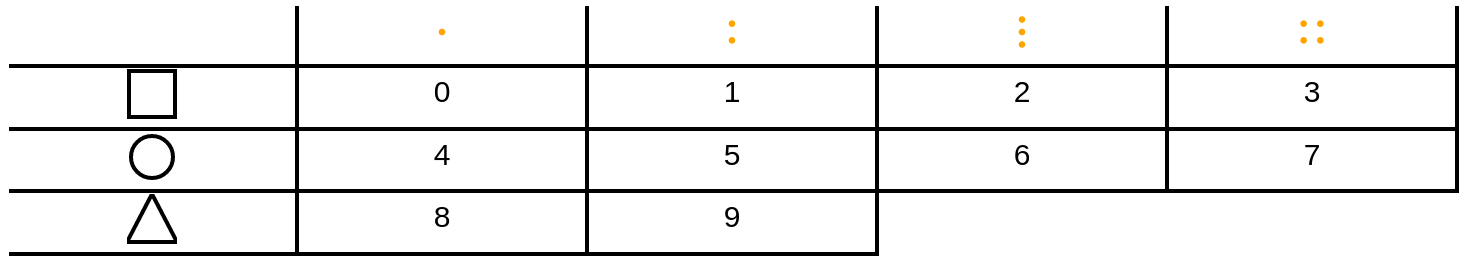
\includegraphics[width=1.0\columnwidth]{figures/symboltable_numbers.png}
    \caption{Symbol table for numbers}
    \label{fig:symboltable_numbers} 
\end{figure}

\subsection{Implementation}

The implementations of the encryption and decryption exercises using symbols are similar to the previous exercises using patterns (figures \ref{fig:symbolDecryption} and \ref{fig:symbolEncryption}). The main difference is the use of a symbol table showing which alphanumerical letter is encrypted with which symbol. A symbol is composed of two shapes. The composition configuration is shown in the symbol table. In the decryption exercise a sequence of symbols is shown. Pupils have to use the symbol table to translate the sequence to its alphanumerical counterpart, decrypting the text. In the encryption exercise, it is the other way around. Pupils have to encrypt a text with the help of the symbol table.

The symbol table is implemented in the \code{SymbolTable.vue} component. It accepts a two-dimensional array representing the table content and generates this table with the help of \code{canvas} elements. Each cell in the table is a \code{canvas} element. Each shape consist of multiple elements, e.g the yellow shape in the top row of the symbol table for numbers (figure \ref{fig:symboltable_numbers}) consists of multiple dots. If there are three or fewer dots, the dots are drawn in a vertical line. For four points, they are drawn in grid style. Other shapes are more complex, like the yellow shapes in the top row of the symbol table for letters (figure \ref{fig:symboltable_letters}), which consists of multiple arcs. The implementation for drawing these shapes takes as an argument the amount of arcs that need to be drawn. It first draws the straight vertical lines and then the specified amount of arcs on this line. This way the implementation can be used for all three arc shapes (listing \ref{lst:drawArcs}) present in the symbol table (figure \ref{fig:symboltable_letters}).

All other shapes are implemented in a similar way, so there is as little code as possible.

\begin{figure} 
    \centering
    
\includegraphics[width=0.4 \columnwidth]{figures/cipher_text.png}
    \caption{Cipher text of an encrypted text} 
    \label{fig:cipher_text} 
\end{figure}

\begin{figure} 
    \centering
    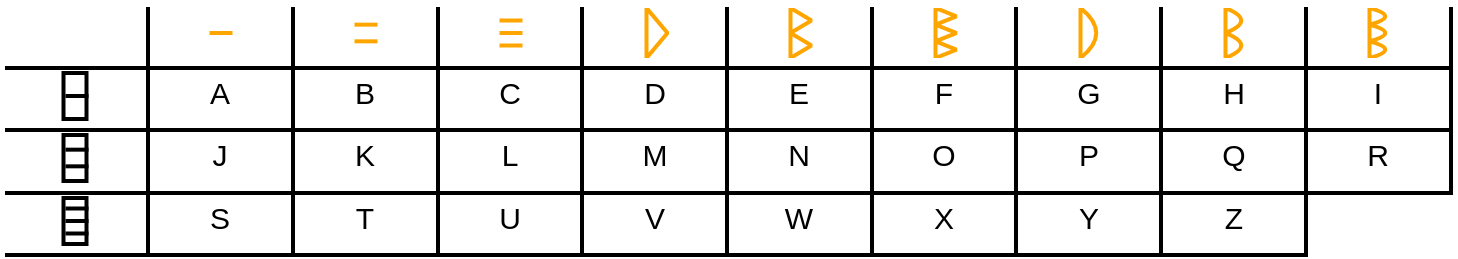
\includegraphics[width=1.0 \columnwidth]{figures/symboltable_letters.png}
    \caption{Symbol table to encrypt and decrypt letters} 
    \label{fig:symboltable_letters} 
\end{figure}

% TC:ignore
\begin{lstlisting}[language=TypeScript,caption={Implementation of drawing a variable amount of arc symbols},label={lst:drawArcs}]
drawArcs(arcs: number) {
  this.ctx.strokeStyle = "#ffa500";
  if (arcs <= 0) {
    return;
  }
  this.ctx.lineJoin = "bevel";
  this.ctx.beginPath();
  this.ctx.moveTo(this.lineWidth / 2, this.height - this.lineWidth / 2);
  this.ctx.lineTo(this.lineWidth / 2, this.lineWidth / 2);
  const diffY = (this.height - this.lineWidth) / (2 * arcs);
  for (let i = 1; i <= arcs; i++) {
    this.ctx.quadraticCurveTo(
      this.width - this.lineWidth / 2,
      (2 * i - 1) * diffY,
      this.lineWidth / 2,
      2 * i * diffY
    );
  }
  this.ctx.stroke();
}
\end{lstlisting}
% TC:endignore

\begin{figure} 
  \centering
  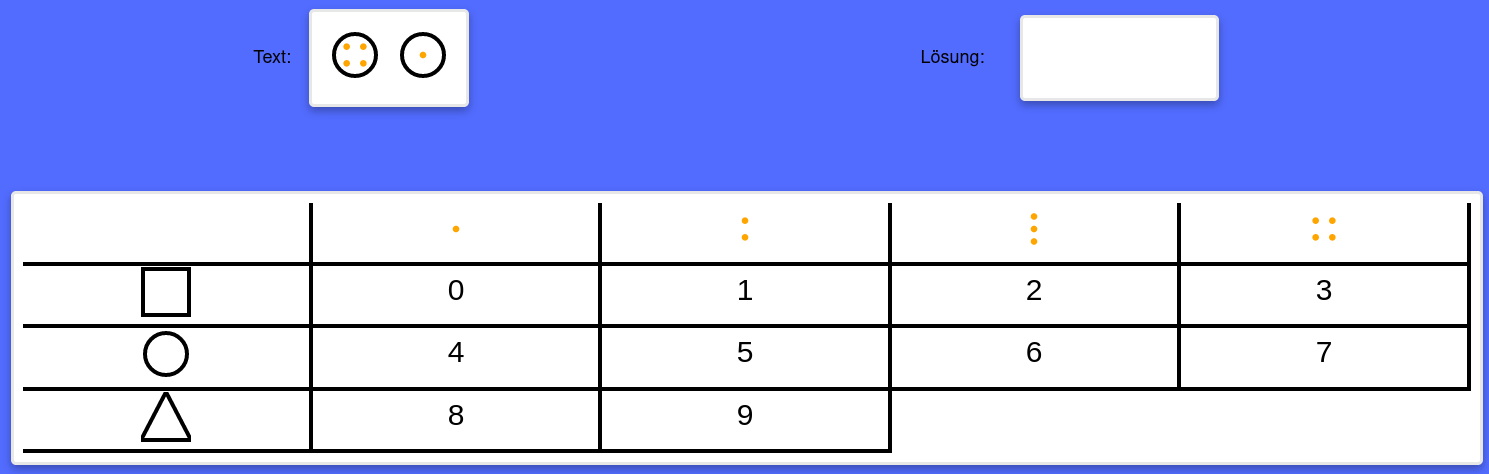
\includegraphics[width=1.0 \columnwidth]{figures/symbol_decrypt.png}
  \caption{Symbol decryption exercise} 
  \label{fig:symbolDecryption} 
\end{figure}

\begin{figure} 
  \centering
  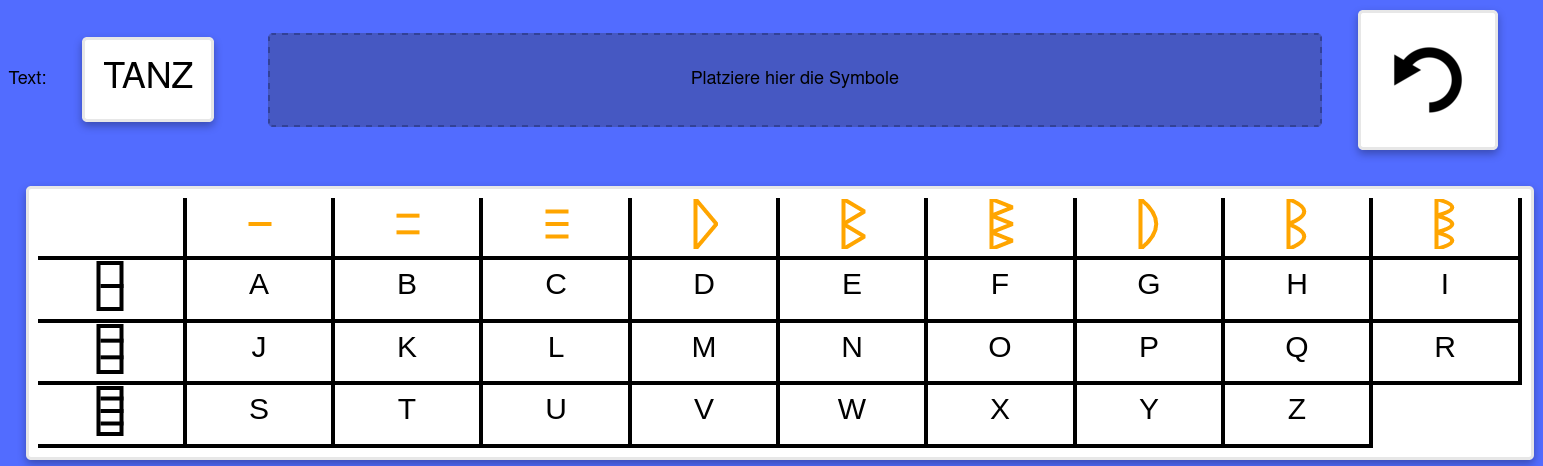
\includegraphics[width=1.0 \columnwidth]{figures/symbol_encrypt.png}
  \caption{Symbol encryption exercise} 
  \label{fig:symbolEncryption} 
\end{figure}
